\documentclass[brazil, notheorems, 10pt]{beamer}
%
%   Arquivo de Configuração dos Slides
%


%
%   Pacotes utilizados
%

% Codificação dos caracteres em formato universal.
\usepackage[utf8]{inputenc}
\usepackage[T1]{fontenc}

% Traduz o texto gerados pelo LaTeX para português. ex.: Capítulo, Seção, Conteúdo.
\usepackage[brazil]{babel}

% Pacotes para ambientes matemáticos
\usepackage{amsmath}
\usepackage{amsthm}
\usepackage{amssymb}

% Diversas funções para o uso das aspas.
\usepackage{csquotes}

% Outros pacotes
\usepackage{hyperref}
\usepackage{tikz}
\usepackage{yfonts}
\usepackage{colortbl}
\usepackage{ragged2e}
\usepackage{helvet}
\usepackage{verbatim}


%
%   Tema
%

% Copyright 2007 by Till Tantau
%
% This file may be distributed and/or modified
%
% 1. under the LaTeX Project Public License and/or
% 2. under the GNU Public License.
%
% See the file doc/licenses/LICENSE for more details.


% Common packages


\usepackage[brazil]{babel}
\usepackage[utf8]{inputenc}
\usepackage{times}
 \mode<article> {
  \usepackage{times}
  \usepackage{mathptmx}
  \usepackage[left=1.5cm,right=6cm,top=1.5cm,bottom=3cm]{geometry}
}

\usepackage{hyperref}
\usepackage[T1]{fontenc}
\usepackage{amsmath,amssymb}
\usepackage{tikz}
\usepackage{colortbl}
\usepackage{yfonts}
\usepackage{colortbl}
\usepackage{translator} % comment this, if not available
\usepackage{ragged2e} % justifying
% Or whatever. Note that the encoding and the font should match. If T1
% does not look nice, try deleting the line with the fontenc.
\usepackage{helvet}
\usepackage{verbatim}


%\usepackage{lipsum}
%\usepackage{enumitem}


\usetheme[
%%% options passed to the outer theme
%    hidetitle,           % hide the (short) title in the sidebar
%    hideauthor,          % hide the (short) author in the sidebar
%    hideinstitute,       % hide the (short) institute in the bottom of the sidebar
%    shownavsym,          % show the navigation symbols
%    width=2cm,           % width of the sidebar (default is 2 cm)
%    hideothersubsections,% hide all subsections but the subsections in the current section
%    hideallsubsections,  % hide all subsections
    right               % right of left position of sidebar (default is right)
%%% options passed to the color theme
%    lightheaderbg,       % use a light header background
  ]{AAUsidebar}

% If you want to change the colors of the various elements in the theme, edit and uncomment the following lines
% Change the bar and sidebar colors:
%\setbeamercolor{AAUsidebar}{fg=red!20,bg=red}
%\setbeamercolor{sidebar}{bg=red!20}
% Change the color of the structural elements:
%\setbeamercolor{structure}{fg=red}
% Change the frame title text color:
%\setbeamercolor{frametitle}{fg=blue}
% Change the normal text color background:
%\setbeamercolor{normal text}{bg=gray!10}
% Highlight the text in the sidebar
\usecolortheme{rose,sidebartab}
% ... and you can of course change a lot more - see the beamer user manual.

% colored hyperlinks
\newcommand{\chref}[2]{%
  \href{#1}{{\usebeamercolor[bg]{AAUsidebar}#2}}%
}


\newcommand{\prn}[1]{\left(#1\right)}

% specify a logo on the titlepage (you can specify additional logos an include them in
% institute command below
\pgfdeclareimage[height=1cm]{titlepagelogo}{theme/figures/ufrn2} % placed on the title page
\pgfdeclareimage[height=1cm]{titlepagelogo2}{theme/figures/imd} % placed on the title page
\titlegraphic{% is placed on the bottom of the title page
  \pgfuseimage{titlepagelogo}
  \hspace{1cm}\pgfuseimage{titlepagelogo2}
}


% Article version layout settings

\mode<article>

\makeatletter
\def\@listI{\leftmargin\leftmargini
  \parsep 0pt
  \topsep 5\p@   \@plus3\p@ \@minus5\p@
  \itemsep0pt}
\let\@listi=\@listI


\setbeamertemplate{frametitle}{\paragraph*{\insertframetitle\
    \ \small\insertframesubtitle}\ \par
}
\setbeamertemplate{frame end}{%
  \marginpar{\scriptsize\hbox to 1cm{\sffamily%
      \hfill\strut\insertshortlecture.\insertframenumber}\hrule height .2pt}}
\setlength{\marginparwidth}{1cm}
\setlength{\marginparsep}{4.5cm}

\def\@maketitle{\makechapter}

\def\makechapter{
  \newpage
  \null
  \vskip 2em%
  {%
    \parindent=0pt
    \raggedright
    \sffamily
    \vskip8pt
    
\includegraphics[width=\linewidth]{theme/figures/imd.png}\par\vskip2em
    {\fontsize{36pt}{36pt}\selectfont Aula \insertshortlecture \par\vskip2pt}
    {\fontsize{24pt}{28pt}\selectfont \color{blue!50!black} \@title\par\vskip4pt}
    %{\Large\selectfont \color{blue!50!black} \insertsubtitle\par}
    \vskip10pt

    \normalsize\selectfont [Notas de Aula]
    Disciplina: \emph{\lecturename \ (\semestre)} \par\vskip1.5em
    \nomedoautor\hskip1em Email: \ \emaildoautor
  }
  \par
  \vskip 1.5em%
}

\let\origstartsection=\@startsection
\def\@startsection#1#2#3#4#5#6{%
  \origstartsection{#1}{#2}{#3}{#4}{#5}{#6\normalfont\sffamily\color{blue!50!black}\selectfont}}

\makeatother

\mode
<all>




% Typesetting Listings

\usepackage{listings}
\lstset{language=Java}

\alt<presentation>
{\lstset{%
  basicstyle=\footnotesize\ttfamily,
  commentstyle=\slshape\color{green!50!black},
  keywordstyle=\bfseries\color{blue!50!black},
  identifierstyle=\color{blue},
  stringstyle=\color{orange},
  escapechar=\#,
  emphstyle=\color{red}}
}
{
  \lstset{%
    basicstyle=\ttfamily,
    keywordstyle=\bfseries,
    commentstyle=\itshape,
    escapechar=\#,
    emphstyle=\bfseries\color{red}
  }
}



% Common theorem-like environments
%\usepackage{amsthm}

\setbeamertemplate{theorems}[numbered]

\theoremstyle{plain}
\newtheorem{Teo}{Teorema}


\theoremstyle{definition}

\newtheorem{Def}[Teo]{Definição}
\newtheorem{exercise}{Exercício}

\theoremstyle{remark}

\newtheorem{Obs}[Teo]{Observação}




\newtheorem{Exer}[Teo]{Exercicio Resolvido}%{\translate{Exercise}}

\newtheorem{Cor}[Teo]{Corolário}
\newtheorem{Exem}[Teo]{Exemplo}
\newtheorem{Lem}[Teo]{Lema}
\newtheorem{Prop}[Teo]{Proposição}
\newtheorem{Sumario}[Teo]{Sumário}
\newtheorem{Obse}{Observação}

\newcounter{Listaexercicios}
\def\Ex#1{
\stepcounter{Listaexercicios} \textbf{\arabic{Listaexercicios}}. #1
}




% New useful definitions:

\newbox\mytempbox
\newdimen\mytempdimen

\newcommand\includegraphicscopyright[3][]{%
  \leavevmode\vbox{\vskip3pt\raggedright\setbox\mytempbox=\hbox{\includegraphics[#1]{#2}}%
    \mytempdimen=\wd\mytempbox\box\mytempbox\par\vskip1pt%
    \fontsize{3}{3.5}\selectfont{\color{black!25}{\vbox{\hsize=\mytempdimen#3}}}\vskip3pt%
}}

\newenvironment{colortabular}[1]{\medskip\rowcolors[]{1}{blue!20}{blue!10}\tabular{#1}\rowcolor{blue!40}}{\endtabular\medskip}

\def\equad{\leavevmode\hbox{}\quad}

\newenvironment{greencolortabular}[1]
{\medskip\rowcolors[]{1}{green!50!black!20}{green!50!black!10}%
  \tabular{#1}\rowcolor{green!50!black!40}}%
{\endtabular\medskip}

%\setbeamertemplate{theorem begin}{{ \inserttheoremheadfont
%\inserttheoremname \inserttheoremnumber
%\ifx\inserttheoremaddition\empty\else\ (\inserttheoremaddition)\fi%
%\inserttheorempunctuation }} \setbeamertemplate{theorem end}{}

\newcommand{\vu}{\vec{u}}
\newcommand{\vv}{\vec{v}}
\newcommand{\vi}{\vec{i}}
\newcommand{\vj}{\vec{j}}
\newcommand{\vk}{\vec{k}}
\newcommand{\vw}{\vec{w}}
\newcommand{\R}{\mathbb{R}}
\newcommand{\N}{\mathbb{N}}
\newcommand{\Z}{\mathbb{Z}}
\newcommand{\Q}{\mathbb{Q}}
\newcommand{\C}{\mathbb{C}}
\newcommand{\U}{\mathcal U}
\newcommand{\I}{\mathcal I}
\newcommand{\sen}{\text{sen}}
\newcommand\seg[2]{\overline{#1#2}}
\def\set#1{\left\{#1\right\}}
\def\paren#1{\left(#1\right)}
\def\colc#1{\left[#1\right]}
\def\modu#1{\left|#1\right|}
\def\tq{\;;\;}
\def\sub#1{\underline{#1}}
\def\link#1#2{\href{#1}{{\tt #2}}}



%
%   Macros
%

\usepackage{macros/macros}


%
%   Ambientes
%

\theoremstyle{plain}
\newtheorem{teorema}{Teorema}

\theoremstyle{definition}
\newtheorem{definicao}[teorema]{Definição}
%\newtheorem{exercicio}{Exercício}

\theoremstyle{remark}
\newtheorem{obs}[teorema]{Observação}
\newtheorem{observacao}[teorema]{Observação}
\newtheorem{corolario}[teorema]{Corolário}
\newtheorem{exemplo}[teorema]{Exemplo}
\newtheorem{lema}[teorema]{Lema}
\newtheorem{proposicao}[teorema]{Proposição}

\newcounter{exercicios}
\newenvironment{exercicio}{\stepcounter{exercicios} \textbf{\arabic{exercicios}}.}{}

% compatibilidade
\newcommand{\Ex}[1]{\begin{exercicio}#1\end{exercicio}}

%
%   Definições e comandos auxiliares do preâmbulo
%

\newcommand{\capitulo}[1]{\lecture[#1]{Capítulo}}
\newcommand{\aula}[1]{\subtitle{#1}}
\newcommand{\autor}{Igor Oliveira}
\newcommand{\email}{\href{mailto:matematicaelementar@imd.ufrn.br}{\texttt{matematicaelementar@imd.ufrn.br}}}
\newcommand{\disciplina}{Matemática Elementar}
\newcommand{\codigo}{IMD1001}

\title{\disciplina}
\date{\today}
\author[\autor]
{
    \autor\\
    \email
}

\def\lecturename{\codigo

\disciplina}

\institute[
	UFRN\\
	Natal-RN
]
{
	Instituto Metrópole Digital\\
	Universidade Federal do Rio Grande do Norte\\
	Natal-RN

}

% compatibilidade
\newcommand{\vu}{\vec{u}}
\newcommand{\vv}{\vec{v}}
\newcommand{\vi}{\vec{i}}
\newcommand{\vj}{\vec{j}}
\newcommand{\vk}{\vec{k}}
\newcommand{\vw}{\vec{w}}
\newcommand{\segmento}[2]{\overline{#1#2}}
\def\colc#1{\left[#1\right]}
\newcommand{\negacao}{\sim}

\justifying

\lecture[10]{Aula}

\def\lecturename{IMD1001
Matemática Elementar}
\def\semestre{2018.1}
\def\nomedoautor{Igor Oliveira}
\def\emaildoautor{\href{mailto:igoroliveira@imd.ufrn.br}{{\tt igoroliveira@imd.ufrn.br}}}

\title[\lecturename]% optional, use only with long paper titles
{Matemática Elementar}

\subtitle{Funções Trigonométricas}  % could also be a conference name

\date{\today}

\author[Igor Oliveira] % optional, use only with lots of authors
{
	\nomedoautor\\
	\emaildoautor
}
% - Give the names in the same order as they appear in the paper.
% - Use the \inst{?} command only if the authors have different
%   affiliation. See the beamer manual for an example

\institute[
%  {\includegraphics[scale=0.2]{aau_segl}}\\ %insert a company, department or university logo
	UFRN\\
	Natal-RN
] % optional - is placed in the bottom of the sidebar on every slide
{% is placed on the title page
	Instituto Metrópole Digital\\
	Universidade Federal do Rio Grande do Norte\\
	Natal-RN

	%there must be an empty line above this line - otherwise some unwanted space is added between the university and the country (I do not know why;( )
}


\begin{document}

\mode<article>
{
\begin{frame} % the plain option removes the sidebar and header from the title page
	\maketitle
\end{frame}

% the titlepage
\begin{frame}[plain,noframenumbering] % the plain option removes the sidebar and header from the title page
	\titlepage
\end{frame}
}

\mode<presentation>
{
% the titlepage
{\imagemfundo
\begin{frame}[plain,noframenumbering] % the plain option removes the sidebar and header from the title page
	\titlepage
\end{frame}}
}

% TOC
\begin{frame}{Índice}{}
\tableofcontents
\end{frame}
%%%%%%%%%%%%%%%%


\section{Introdução}

\begin{frame} \frametitle{Apresentação da Aula}

A trigonometria é estudada desde os gregos e sua motivação inicial
era determinar os seis elementos principais do triângulo (seus lados
e ângulos) quando conhecidos alguns deles.

Com a criação do Cálculo Infinitesimal veio a necessidade da criação
%de funções trigonométricas definidas em $\R$, conforme estudaremos
nessa aula.

Tais funções ganharam notoriedade quando, em 1822, Joseph Fourier
provou que toda função periódica é uma soma (finita ou infinita) de
%funções do tipo $a\cos (nx) +b \sen (nx)$. Tal descoberta deu origem
a toda uma área da matemática, a Análise de Fourier. Além disso,
segundo o banco de dados da revista "Mathematical Reviews", o nome
mais citado nos títulos de trabalhos matemáticos nos últimos 50 anos
é o de Fourier.

\end{frame}

%------------------------------------------------------------------------------------------------------------
\def\cos{cos}
\section{Trigonometria no Triângulo Retângulo}
\begin{frame} \frametitle{Definição}
\begin{Def}
Em um triângulo retânglulo $ABC$ como na figura abaixo, define-se o
\sub{cosseno} ($\cos$) e o \sub{seno} (sen) dos ângulos agudos do
triângulo:
\begin{center}
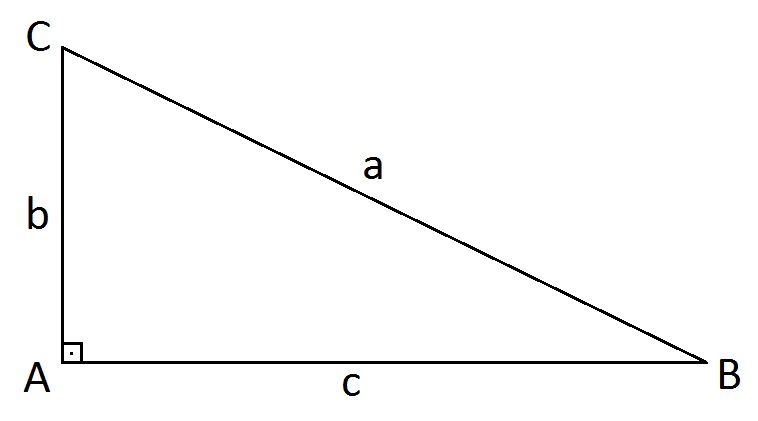
\includegraphics[width=4.8cm]{figures/triangret.jpg}
\end{center}
$$\cos \widehat B = \frac c a = \frac {\text{cateto
adjacente}}{hipotenusa}, \ \ \ \ \sen \widehat B = \frac b a = \frac
{\text{cateto oposto}}{hipotenusa},$$
$$\cos \widehat C = \frac b a \ \ \ \ \text{e} \ \ \ \ \sen \widehat
C = \frac c a.$$
\end{Def}



\end{frame}

%------------------------------------------------------------------------------------------------------------

\begin{frame}
\frametitle{Propriedades} %\framesubtitle{Exemplos}
As relações definidas dessa maneira são únicas para cada ângulo em
decorrência da proporcionalidade dos lados de triângulos
semelhantes. Portanto, calcula-se o seno e o cosseno de um ângulo
independentemente do triângulo retângulo que o contém.

\begin{Prop}
\begin{itemize}
	\item O cosseno de um ângulo agudo é igual ao seno do seu
	complementar e vice-versa. Daí a palavra "cosseno" (seno do
	complemento);
	\item O seno e o cosseno são números compreendidos entre 0 e 1 por
	serem razões entre um cateto pela hipotenusa de um triângulo
	retângulo.
\end{itemize}
\end{Prop}




\end{frame}

%------------------------------------------------------------------------------------------------------------

\begin{frame}
\frametitle{Relação Fundamental da Trigonometria} %\framesubtitle{Exemplos}

\begin{Prop}[Relação Fundamental da Trigonometria]
Seja $\widehat B$ um dos ângulos agudos de um triângulo retângulo
cuja hipotenusa mede $a$ e os catetos, $b$ e $c$. Então:
$$\sen^2 \widehat B + \cos^2 \widehat B = 1.$$
\end{Prop}
\end{frame}

%------------------------------------------------------------------------------------------------------------
\section{Atividade Online}
\begin{frame}
\frametitle{Atividade Online} %\framesubtitle{Exemplos}

\href{https://pt.khanacademy.org/math/trigonometry/trigonometry-right-triangles/intro-to-the-trig-ratios/e/trigonometry_1}
{{\tt Atividade 19 - Razões Trigonométricas em Triângulos
Retângulos}}

\href{https://pt.khanacademy.org/math/trigonometry/trigonometry-right-triangles/trig-solve-for-a-side/e/trigonometry_2}
{{\tt Atividade 20 - Como Calcular a Medida de um Lado em Triângulos
Retângulos }}


Veja o desempenho na Missão Trigonometria.


\end{frame}

%------------------------------------------------------------------------------------------------------------
\section{Funções Trigonométricas}
\begin{frame}
\frametitle{O Círculo Trigonométrico} %\framesubtitle{Exemplos}

A relação fundamental $\sen^2 \widehat B + \cos^2 \widehat B = 1$
sugere que os pontos do plano cartesiano $\paren{\cos \widehat B,
\sen \widehat B}$ pertencem a uma circunferência de raio 1, como
mostra a figura abaixo.
\begin{center}
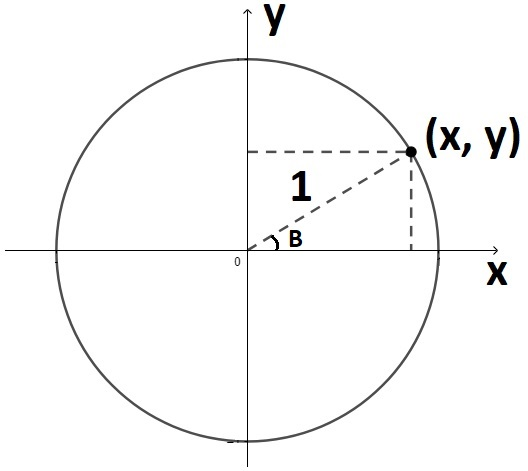
\includegraphics[width=4.5cm]{figures/circtrigB.jpg}
\end{center}

Dessa forma, sendo $\widehat B$ o ângulo medido a partir do eixo
positivo de $x$ e tomando o sentido anti-horário como sentido
positivo, os pontos $(x, y)$ do círculo acima são tais que $x = \cos
\widehat B$ e $y = \sen \widehat B$.


\end{frame}



%------------------------------------------------------------------------------------------------------------

\begin{frame}
\frametitle{O Círculo Trigonométrico} %\framesubtitle{Exemplos}

Agora, a fim de definirmos as funções trigonométricas como funções
reais, considere a seguinte função, chamada de função de Euler: $E:
\R \to \R^2$ tal que $E(t)$ é o ponto $(x, y)$ do círculo
trigonométrico obtido após ``enrolarmos'', com corda de comprimento
$t$, o círculo trigonométrico iniciando no ponto $(1, 0)$ e tomando
como sentido positivo o sentido anti-horário.
\begin{center}
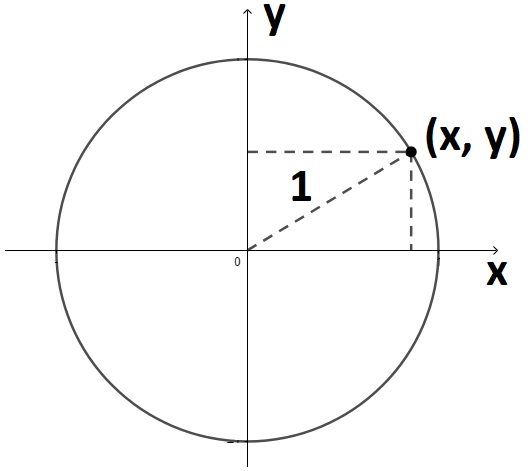
\includegraphics[width=5cm]{figures/circtrig.jpg}
\end{center}
\end{frame}



%------------------------------------------------------------------------------------------------------------

\begin{frame}
\frametitle{O Círculo Trigonométrico} %\framesubtitle{Exemplos}

\begin{Def}
As funções $\cos : \R \to \R$ e $\sen : \R \to \R$, chamadas
\sub{função cosseno} e \sub{função seno} respectivamente, são
definidas pondo-se, para cada $t \in \R$,
$$E(t) = \paren{\cos t , \sen t}.$$
\end{Def}
Em outras palavras, $x= \cos t$ e $y = \sen t$ são, respectivamente,
a abcissa e a ordenada do ponto $E(t)$ da circunferência unitária.

\end{frame}



%------------------------------------------------------------------------------------------------------------
\section{Propriedades das Funções Seno e Cosseno}
\begin{frame}
\frametitle{Propriedades} %\framesubtitle{Exemplos}


Considere as seguintes definições acerca de funções reais.

\begin{Def}
Uma função $f: \R \to \R$ chama-se \sub{periódica} quando existe $T
\in \R^\ast$ tal que $f(t + T) = f(t)$ para todo $t \in \R$. Ao
menor número $T>0$ que faz a propriedade anterior ser satisfeita,
damos o nome de \sub{período} da função $f$.
\end{Def}\pause
Como uma volta completa no círculo trigonométrico tem $2 \pi$ de
comprimento, é fácil ver que a função seno e cosseno são periódicas
de período $2\pi$.
\end{frame}
%------------------------------------------------------------------------------------------------------------

\begin{frame}
\frametitle{Propriedades} %\framesubtitle{Exemplos}

\begin{Def}
Uma função $f: \R \to \R$ é \sub{par} quando se tem $f(-t) = f(t)$
para todo $t\in \R$. Se for o caso de $f(-t) = - f(t)$ para todo $t
\in \R$, dizemos que $f$ é \sub{ímpar}.
\end{Def}\pause

\begin{Prop}
A função seno é ímpar e a função cosseno é par.
\end{Prop}


\end{frame}
%------------------------------------------------------------------------------------------------------------

\begin{frame}
\frametitle{Propriedades} %\framesubtitle{Exemplos}

Segue imediatamente da definição das funções trigonométricas que a
relação fundamental $$ \sen^2 t + \cos^2 t = 1$$ vale para todo $t
\in \R$. \\
Além disso, valem as seguintes igualdades para todo $t \in \R$:
\begin{center}
\begin{tabular}{ c c }
		%\hline
		% after \\: \hline or \cline{col1-col2} \cline{col3-col4} ...
		$\cos \paren{t+ \pi} = -\cos t$, & $\sen \paren{t+ \pi} = -\sen t$, \\
		$\cos \paren{t+ \frac {\pi} 2} = -\sen t$, & $\sen \paren{t+ \frac {\pi} 2} = \cos t$, \\
		$\cos \paren{ \frac {\pi} 2 -t} = \sen t$, & $\sen \paren{ \frac {\pi} 2 -t} = \cos t$, \\
		$\cos \paren{ \pi -t} = -\cos t$, & $\sen \paren{ \pi -t} = \sen t$. \\
		%\hline
	\end{tabular}
\end{center}

\end{frame}

%------------------------------------------------------------------------------------------------------------
\section{Atividade Online}
\begin{frame}
\frametitle{Atividade Online} %\framesubtitle{Exemplos}

\href{https://pt.khanacademy.org/math/trigonometry/unit-circle-trig-func/trig-values-special-angles/e/trigonometric-functions-of-special-angles}
{{\tt Atividade 21 - Valores Trigonométricos de Ângulos Especiais}}

\href{https://pt.khanacademy.org/math/trigonometry/unit-circle-trig-func/pythagorean-identity/e/circles-and-pythagorean-identities}
{{\tt Atividade 22 - Use a Identidade Trigonométrica Fundamental}}

\href{https://pt.khanacademy.org/math/trigonometry/trig-equations-and-identities/basic-sinusoidal-equations/e/solve-basic-sinusoidal-equations}
{{\tt Atividade 23 - Resolva Equações Senoidais (Básico)}}


Veja o desempenho na Missão Trigonometria.


\end{frame}
%------------------------------------------------------------------------------------------------------------
\section{Gráficos das Funções Seno e Cosseno}
\begin{frame}
\frametitle{Gráfico da Função Cosseno} %\framesubtitle{Exemplos}

\begin{Exem}
O gráfico da função $\cos : \R \to \R$ é dado por:
\begin{center}
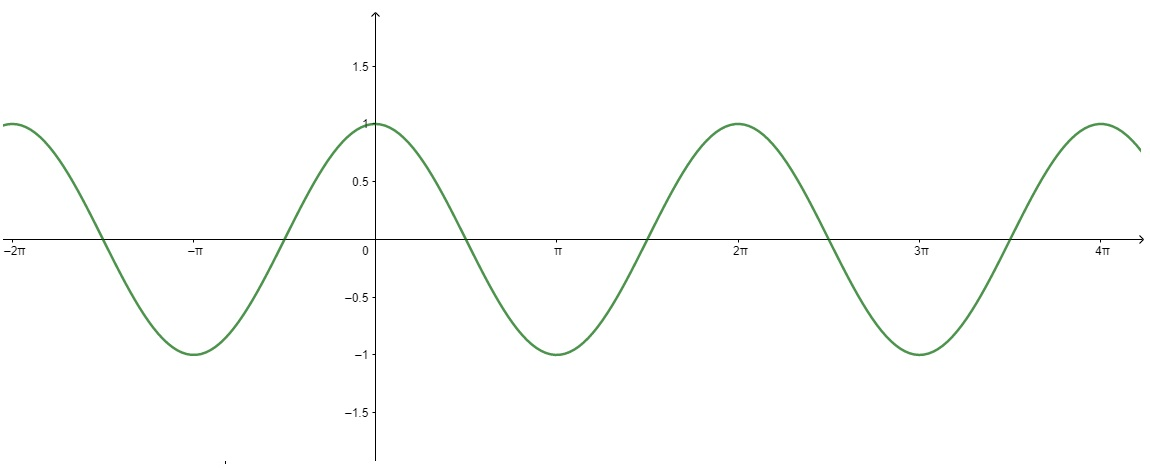
\includegraphics[width=9.9cm]{figures/grafcos.jpg}
\end{center}
\end{Exem}

\end{frame}




%------------------------------------------------------------------------------------------------------------
\begin{frame}
\frametitle{Gráfico da Função Seno} %\framesubtitle{Exemplos}

\begin{Exem}
O gráfico da função $\sen: \R \to \R$ é dado por:
\begin{center}
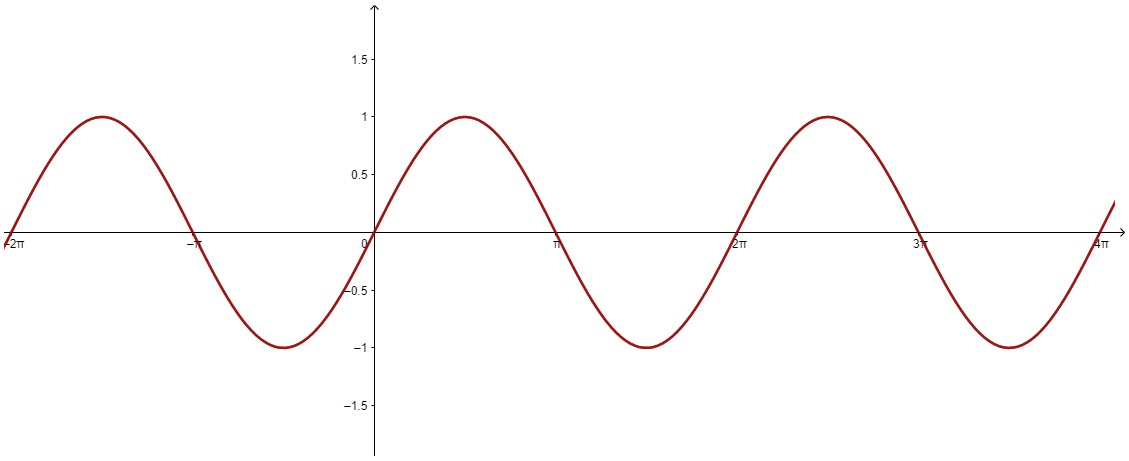
\includegraphics[width=9.9cm]{figures/grafsen.jpg}
\end{center}
\end{Exem}

\end{frame}

%------------------------------------------------------------------------------------------------------------
\section{Atividade Online}
\begin{frame}
\frametitle{Atividade Online} %\framesubtitle{Exemplos}

\href{https://pt.khanacademy.org/math/trigonometry/trig-function-graphs/graphing-sinusoids/e/graphs_of_sine_and_cosine}
{{\tt Atividade 24 - Gráfico de Funções Senoidais}}



Veja o desempenho na Missão Trigonometria.


\end{frame}
%------------------------------------------------------------------------------------------------------------
\section{Outras Funções Trigonométricas}
\begin{frame}
\frametitle{Definições} %\framesubtitle{Exemplos}

\begin{Def}\label{outrasfunctrig}
Definem-se, através das funções seno e cosseno, as funções
trigonométricas com as seguintes leis de formação:
\begin{itemize}
	\item $\tan x = \frac {\sen x}{\cos x}$, \sub{tangente};
	\item $\cot x = \frac {\cos x}{\sen x}$, \sub{cotangente};
	\item $\sec x = \frac {1}{\cos x}$, \sub{secante};
	\item $\csc x = \frac {1}{\sen x}$, \sub{cossecante}.
\end{itemize}
Os domínios dessas funções não contêm o conjunto dos valores de $x$
que zeram seus respectivos denominadores.
\end{Def}
Por exemplo, o maior subconjunto dos reais no qual podemos definir
as funções tangente e secante é $$\bigcup_{k \in \Z} \paren{k \pi -
\frac {\pi} 2, k \pi + \frac {\pi} 2}.$$
\end{frame}
%------------------------------------------------------------------------------------------------------------

\begin{frame}
\frametitle{Gráfico da Função Tangente} %\framesubtitle{Exemplos}

\begin{Exem}
O gráfico da função $\tan: \bigcup_{k \in \Z} \paren{k \pi - \frac
{\pi} 2, k \pi + \frac {\pi} 2} \to \R$ é:
\begin{center}
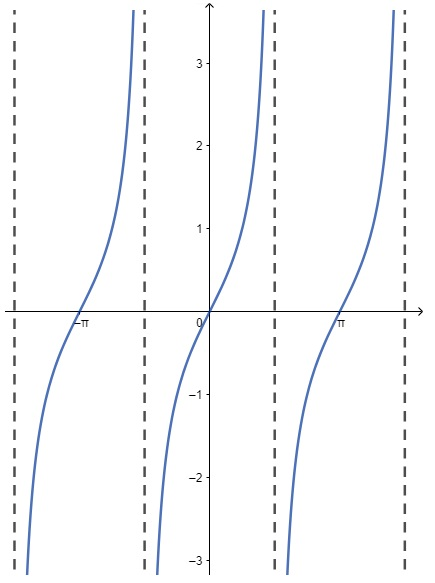
\includegraphics[width=4.6cm]{figures/graftan.jpg}
\end{center}
\end{Exem}

\end{frame}

%------------------------------------------------------------------------------------------------------------

\begin{frame}
\frametitle{Propriedades da Função Tangente} %\framesubtitle{Exemplos}

\begin{Prop}
Valem as seguintes propriedades acerca da função tangente:
\begin{itemize}
	\item Embora não seja definida para todo número real, a função
	tangente pode ser considerada uma função periódica de período
	$\pi$ em todo o seu domínio, pois $\tan \paren{x+\pi} = \tan x$;
	\item Para todo par de pontos  $(x_1, y_1)$ e $(x_2, y_2)$ em uma reta não vertical, com $x_1 \neq x_2$, se
	$\alpha$ é o ângulo formado pela reta e o eixo $x$, então $$\tan
	\alpha = \frac {y_2 - y_1} {x_2 - x_1}.$$
	\item Ao definirmos $tan: \paren{- \frac {\pi} 2, \frac {\pi} 2} \to \R$,
obtemos uma bijeção. Assim, o intervalo aberto $\paren{- \frac {\pi}
2, \frac {\pi} 2}$ tem a mesma cardinalidade que $\R$.

\end{itemize}
\end{Prop}


\end{frame}

%------------------------------------------------------------------------------------------------------------

\begin{frame}
\frametitle{A Função Inversa da Tangente}  %\framesubtitle{Exemplos}


\begin{Exem}
Como $tan: \paren{- \frac {\pi} 2, \frac {\pi} 2} \to \R$ é
bijetiva, então essa função possui inversa, que chamamos de
\sub{arco tangente} e denotamos por $\arctan : \R \to
\paren{- \frac {\pi} 2, \frac {\pi} 2}$. Seu gráfico é
\begin{center}
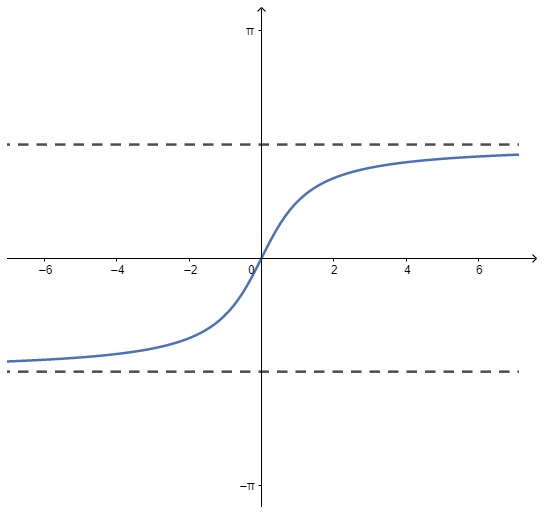
\includegraphics[width=5.5cm]{figures/grafarctan.jpg}
\end{center}
\end{Exem}


\end{frame}

%------------------------------------------------------------------------------------------------------------
\section{Atividade Online}
\begin{frame}
\frametitle{Atividade Online} %\framesubtitle{Exemplos}



\href{https://pt.khanacademy.org/math/trigonometry/trigonometry-right-triangles/reciprocal-trig-ratios/e/reciprocal_trig_funcs}
{{\tt Atividade 25 - Razões Trigonométricas Recíprocas}}

\href{https://pt.khanacademy.org/math/trigonometry/trigonometry-right-triangles/modeling-with-right-triangles/e/applying-right-triangles}
{{\tt Atividade 26 - Problemas com Triângulos Retângulos}}


Veja o desempenho na Missão Trigonometria.


\end{frame}

%------------------------------------------------------------------------------------------------------------
\section{Seno e Cosseno da Soma}
\begin{frame}
\frametitle{Fórmulas de Adição de Arcos} %\framesubtitle{Exemplos}

\begin{Prop}
Sejam $\alpha, \beta \in \R$. Então
$$\cos \paren{\alpha + \beta} = \cos \alpha \cdot \cos \beta - \sen
\alpha \cdot \sen \beta$$ e
$$\sen \paren{\alpha + \beta} = \sen \alpha \cdot \cos \beta +\sen \beta \cdot
\cos \alpha.$$
\end{Prop}\pause
Da paridade das funções seno e cosseno seguem que:
$$\cos \paren{\alpha - \beta} = \cos \alpha \cdot \cos \beta + \sen
\alpha \cdot \sen \beta$$ e
$$\sen \paren{\alpha - \beta} = \sen \alpha \cdot \cos \beta - \sen \beta \cdot
\cos \alpha.$$

Além disso, temos os casos particulares
$$\cos \paren{2\alpha } = \cos^2 \alpha  - \sen^2 \alpha \ \ \text{ e }
\ \ \sen \paren{2\alpha } = 2\sen \alpha \cdot \cos \alpha.$$ As
fórmulas acima valem para todo $\alpha, \beta \in \R$.


\end{frame}

%------------------------------------------------------------------------------------------------------------
\begin{frame}
\frametitle{Rotação de Pontos no Plano Cartesiano} %\framesubtitle{Exemplos}

Considere o ponto $A = (x, y) \in \R^2$ e chame de $\alpha$ o ângulo
formado pelo segmento $OA$ com o eixo positivo de $x$. A função
$T_{\theta} : \R^2 \to \R^2$  tal que
$$T_{\theta}\paren{x, y} = \paren{x\cdot \cos \theta - y\cdot \sen \theta, x\cdot \sen \theta + y\cdot \cos
\theta}$$ é a rotação de ângulo $\theta$ do ponto $A = (x,y)$ em
torno da origem.

\begin{center}
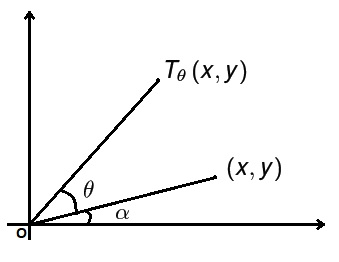
\includegraphics[width=5.5cm]{figures/rotacao.jpg}
\end{center}


\end{frame}

%------------------------------------------------------------------------------------------------------------
\section{Atividade Online}
\begin{frame}
\frametitle{Atividade Online} %\framesubtitle{Exemplos}



\href{https://pt.khanacademy.org/math/trigonometry/trig-equations-and-identities/intro-to-trig-angle-addition-identities/e/trig_addition_identities}
{{\tt Atividade 27 - Uso das Identidades Trigonométricas de Soma de
Ângulos}}

\href{https://pt.khanacademy.org/math/trigonometry/trig-equations-and-identities/using-trig-identities/e/applying-angle-addition-formulas}
{{\tt Atividade 28 - Calcule Valores Trigonométricos a Partir de
Identidades de Soma de Ângulos}}


Veja o desempenho na Missão Trigonometria.


\end{frame}




%------------------------------------------------------------------------------------------------------------

\section{Lei dos Cossenos e Lei dos Senos}
\begin{frame}
\frametitle{Lei dos Cossenos} %\framesubtitle{Exemplos}

\begin{Teo}[Lei dos Cossenos]
Seja $ABC$ um triângulo com $a = \segmento BC$, $b = \segmento AC$ e $c = \segmento
AB$. Então
$$b^2 = a^2 + c^2 - 2 ac \cdot \cos \widehat B.$$
\end{Teo}
A Lei dos Cossenos é uma generalização do Teorema de Pitágoras. Note
que, se $\widehat B$ é um ângulo reto, então $\cos \widehat B = 0$ e
$b$ será a hipotenusa do triângulo.
\end{frame}

%------------------------------------------------------------------------------------------------------------



\begin{frame}
\frametitle{Lei dos Senos} %\framesubtitle{Exemplos}

\begin{Teo}[Lei dos Senos]
Seja $ABC$ um triângulo com $a = \segmento BC$, $b = \segmento AC$ e $c = \segmento
AB$. Então
$$\frac a {\sen \widehat A} = \frac b {\sen \widehat B} = \frac c {\sen \widehat C}$$
\end{Teo}
A Lei dos Senos nos diz que, em todo triângulo, a razão entre um
lado e o seno do ângulo oposto é constante.\pause

As leis dos cossenos e dos senos permitem obter os seis elementos de
um triângulo quando são dados três deles, desde que um seja lado,
conforme os casos clássicos de congruência de triângulos.


\end{frame}



%------------------------------------------------------------------------------------------------------------
\section{Atividade Online}
\begin{frame}
\frametitle{Atividade Online} %\framesubtitle{Exemplos}

\href{https://pt.khanacademy.org/math/trigonometry/trig-with-general-triangles/solving-general-triangles/e/law-of-sines-and-cosines-word-problems}
{{\tt Atividade 29 - Problemas com Triângulos Gerais }}


Veja o desempenho na Missão Trigonometria.


\end{frame}


%------------------------------------------------------------------------------------------------------------

\section{Exercícios}
\begin{frame}
\frametitle{Exercícios} %\framesubtitle{Exemplos}
\Ex{Na Definição 1 definimos seno e cosseno de um ângulo no
triângulo retângulo. Como você definiria, com os lados de um
triângulo retângulo, as demais relações trigonométricas da Definição
\ref{outrasfunctrig}?}

\Ex{Saber para quais valores $t$ são válidas algumas equações
envolvendo equações trigonométricas é muito importante. Determine o
conjunto solução de cada uma das equações abaixo:
\begin{enumerate}[(a)]
	\item $\sen t = 0$, $\cos t = 0$ e $\tan t = 0$;
	\item $\sen t = 1$, $\cos t = 1$;
	\item $\sen t = -1$, $\cos t = -1$ e $\tan t = -1$;
	\item $\sen t = \cos t$ e $\tan t = 1$;
	\item $\csc t = 0$, $\sec t = 0$ e $\cot t = 0$;
	\item $\csc t = 1$, $\sec t = 1$;
	\item $\csc t = -1$, $\sec t = -1$ e $\cot t = -1$;
	\item $\csc t = \sec t$ e $\cot t = 1$.
\end{enumerate}
}

\end{frame}


%------------------------------------------------------------------------------------------------------------

\begin{frame}
\frametitle{Exercícios} %\framesubtitle{Exemplos}


\Ex{A figura abaixo representa o gráfico da função $f_1 : \R \to
\R$, $f_1(x) = x \cdot \sen x$, traçado no intervalo $\colc{-20 \pi,
20 \pi}$, juntamente com as retas $y=x$ e $y=-x$.
\begin{center}
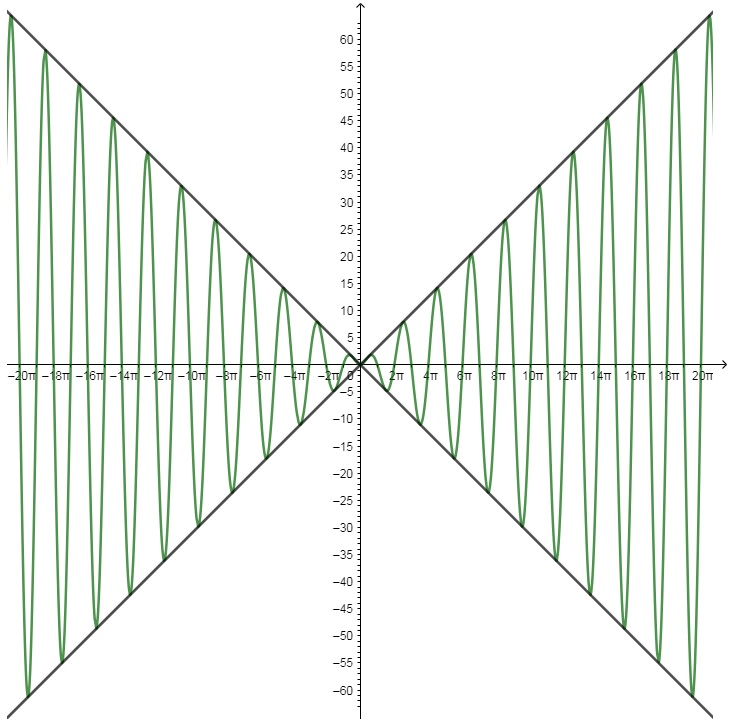
\includegraphics[width=2.5cm]{figures/grafxsenx.jpg}
\end{center}
\begin{enumerate}[(a)]
	\item Explique por que o gráfico de $f_1$ fica limitado entre
	essas retas e indique todos os pontos em que o gráfico toca as retas;
	\item Considere a seguinte afirmação: \emph{Os máximos e
	mínimos locais da função $f_1$ ocorrem nos mesmos valores
	de $x$ que os da função seno.} Esta afirmação é verdadeira?
	\item Como você espera visualizar o gráfico da função $f_2: \R \to
	\R$, definida por $f_2(x) = x^2 \cdot \sen x$?
\end{enumerate}}
%\Ex{Dada as PA's $\paren{a_1, a_2, \dots, a_n, \dots}$ e
%$\paren{b_1, b_2, \dots, b_n, \dots}$, mostre que existe uma, e
%somente uma, função afim $f: \R \to \R$ tal que $f(a_1) = b_1$,
%$f(a_2) = b_2$, \dots , $f(a_n) = b_n$, \dots}
\end{frame}

%------------------------------------------------------------------------------------------------------------

\begin{frame}
\frametitle{Exercícios} %\framesubtitle{Exemplos}

\Ex{Na figura abaixo, os segmentos $AD$ e $OD$ representam,
respectivamente, $\tan x$ e $\sec x$.
\begin{center}
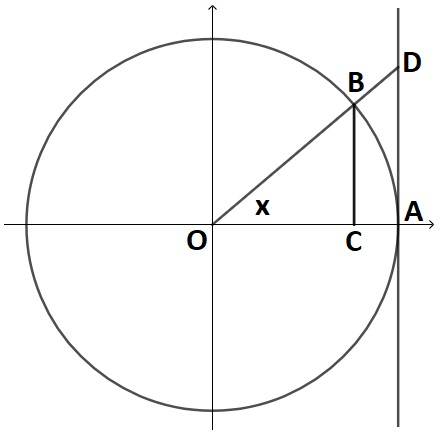
\includegraphics[width=4.5cm]{figures/circtansec.jpg}
\end{center}
\begin{enumerate}[(a)]
	\item Justifique a afirmação acima;
	\item Qual a interpretação dos sinais de $\tan x$ e $\sec x$ na
	figura?
	\item Faça uma figura análoga para representar $\cot x$ e $\csc
	x$, justificando a construção.
\end{enumerate}}


\end{frame}


%------------------------------------------------------------------------------------------------------------

\begin{frame}
\frametitle{Exercícios} %\framesubtitle{Exemplos}

\Ex{Encontre as três menores soluções positivas da equação $$\cos
\paren{3x - \frac {\pi} 4} = 0.$$}

\Ex{Mostre que o perímetro do pentágono regular inscrito em um
círculo unitário é dado por $10\sen \frac {\pi} 5$.}

\Ex{Considere a função $f: \R \to \R$ definida por $f(x) = \sen
\paren{ax}+\sen \paren{bx}$, em que $a$ e $b$ são constantes reais.
\begin{enumerate}[(a)]
	\item Mostre que, se $a$ e $b$ são racionais, então $f$ é
	periódica;\\
	\emph{Dica:} Mostre que o período de $\sen \paren{ax}$ é $\frac
	{2\pi} a$.
	\item A recíproca da afirmação do item anterior é verdadeira?
	Justifique sua resposta.
\end{enumerate}}

\end{frame}



%------------------------------------------------------------------------------------------------------------


\begin{frame}
\frametitle{Exercícios} %\framesubtitle{Exemplos}

\Ex{Prove as identidades abaixo, válidas para todo $x$ onde as
expressões estão definidas:
\begin{enumerate}[(a)]
	\item $\frac{1-\tan^2 x}{1+\tan^2 x} = 1 - 2\sen^2 x$;
	\item $\frac{\cos x - \sen x}{\cos x + \sen x} = \frac{1 - \tan x}{1+\tan
	x}$;
	\item $\frac{\sen x}{\csc x - \cot x} = 1+ \cos x$;
	\item $\cos^2 x = \frac {1+\cos \paren{2x}} 2$;
	\item $\sen^2 x = \frac {1-\cos \paren{2x}} 2$;
	\item $\frac{1-\tan^2 x}{1+\tan^2 x} = \cos^2 x - \sen^2 x = \cos \paren{2x}$;
	\item $\frac{2\tan x}{1+\tan^2 x} = 2\sen x \cos x= \sen\paren{2x}$.
\end{enumerate}}

\end{frame}



%------------------------------------------------------------------------------------------------------------

\begin{frame}
\frametitle{Exercícios} %\framesubtitle{Exemplos}

\Ex{Use as fórmulas de seno e cosseno da soma para determinar os
senos e cossenos dos seguintes ângulos (medidos em radianos): $\frac
{\pi} 8$, $\frac{\pi} {12}$, $\frac {3\pi} 8$ e $\frac{5\pi}{12}$.}

\Ex{Obtenha fórmulas para $\tan\paren{\alpha + \beta}$ e para
$\sec\paren{\alpha + \beta}$, em função de $\tan \alpha$ e $\tan
\beta$.}

\end{frame}

%------------------------------------------------------------------------------------------------------------

\section{Bibliografia}

\frame{
	\frametitle{Bibliografia}
	\begin{thebibliography}{99}
		\bibitem {label1}
		CARMO, Manfredo Perdigão; MORGADO, Augusto César; WAGNER, Eduardo.
		\newblock \emph{Trigonometria - Números Complexos}.
		\newblock 3. ed. Rio de Janeiro: SBM, 2005.
	\end{thebibliography}
}

\end{document}
